\chapter{Introduction}

The path planning problem consists of moving a mobile robot platform or end-effector from a start location to a goal location.
Examples vary from ground robots moving through an office building, UAVs navigating to GPS waypoints, or end-effectors avoiding objects on a cluttered table to grasp an object.
Methods of solving such a problem depend largely on the construction and knowledge of the environment and the knowledge the robot has about its position within the environment. For example, a mobile robot operating in the plane within a static environment, \textit{a priori} map, and direct position sensing has different challenges than a mobile robot operating in three-dimensions, within an unknown dynamic environment, and only platform velocity estimation.
Popular approaches include graph search algorithms such as A* or D*, Bug algorithms, and potential fields approaches. Potential fields algorithms treat the mobile robot as a point mass that is repelled by obstacles and attracted by the goal. The algorithm detailed here 

The problem considered in here is that of a mobile robot operating in the plane in an unknown static office-like environment with range and bearing estimate to a goal location. The robot also estimates the range and bearing to occlusions in the environment.

\begin{figure}[h]
	\centering
	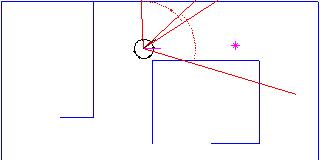
\includegraphics{sim_fig1.jpg}
	\caption[Planar robot simulation example.]
	{Planar robot simulation example. The robot is indicated by a black circle with the red cones simulating ultrasonic sensor beams and their detected range indicated by dotted red arcs in the red cone. Blue lines represent obstacles. The magenta line points towards the goal location, which is indicated by a magenta star.}
	\label{fig:simFig1}
\end{figure}




